\documentclass[a4paper,12pt]{article}
\usepackage[polish]{babel}
\usepackage[utf8]{inputenc}
\usepackage[T1]{fontenc}
\usepackage{latexsym}
\usepackage[usenames,dvipsnames]{xcolor}
\usepackage{graphicx}
\usepackage{fancyhdr}
\usepackage{chngpage}
\usepackage{enumerate}
\usepackage{enumitem}
\usepackage{listings}
\usepackage{geometry}
\usepackage{lscape}

\usepackage{color}
\usepackage{array}
\usepackage{supertabular}
\usepackage{hhline}
\usepackage{hyperref}

\linespread{1.5}
\pagestyle{fancy}
\geometry{lmargin=3cm, rmargin=3cm, bmargin=3cm, tmargin=3cm}

\lhead{}

\title
{
	\Large
	Akademia Górniczo-Hutnicza im. Stanisława Staszica \\ w Krakowie \\
	\vspace{15 mm} 	
	Zaawansowane techniki integracji systemów \\ 
	\textbf{ Platforma wymiany dóbr pomiędzy podmiotami realizującymi proces produkcji } \\
	\vspace{15 mm}
	
\includegraphics[scale=0.8]{gfx/agh.jpg}	
	\vspace{5 mm}
}
\author
{
	\begin{tabular}{cc}
	Krzysztof Mycek & Mateusz Rudnicki \\ 
	Jakub Krawętkowski & Jarosław Szczęśniak \\ 
	\end{tabular} 
	\vspace{10 mm}
}

\begin{document}

\maketitle

\pagebreak

\tableofcontents

\newpage

\lstset{basicstyle=\footnotesize, columns=fullflexible}

\section{Cel projektu}

Celem projektu jest stworzenie platformy wymiany dóbr między producentami i konsumentami, umożliwiającej między innymi negocjacje i renegocjacje kontraktów. Docelowo przebiegiem wymiany dóbr mają zarządzać algorytmy orkiestracji i choreografii.

\newpage

\section{Realizacja}

\subsection{Wstęp}

W ramach projektu stworzyliśmy platformę systemu wymiany dóbr. W obrębie systemu udało nam się zaimplementować kluczowe klasy i funkcjonalności, a także dokonać integracji technologii odpowiedzialnych za sterowanie i wspomaganie procesu wymiany dóbr – JADE i JMX. Stworzona platforma stanowi doskonałą bazę do rozszerzania i dodania algorytmów choreografii i orkiestracji których nie udało nam się zaimplementować w wyniku ograniczeń czasowych.

\newpage

\subsection{Narzędzia}

\textbf{JADE} - platforma agentowa wpełni napisana w języku JAVA upraszczająca tworzenie systemów wieloagentowych. Jedna z najbardziej popularnych platform Open Source. Posiada duże zaplecze i wsparcie techniczne \cite{jade}.
\\ \\
\textbf{JMX} - technologia umożliwiająca zarządzanie oraz monitorowanie aplikacji i usług sieciowych \cite{jmx}.
\\ \\
\textbf{JADEMX} - Środowisko łączące obie technologie, dzięki któremu agenci JADE mogą udostępniać swoje atrybuty i funkcje w sposób zgodny z JMX \cite{jademx}.
\\ \\
\textbf{Eclipse} - wielojęzykowe, zintegrowane środowisko programistyczne \cite{eclipse}.
\\ \\
\textbf{XStream} - biblioteka umożliwająca serializację obietów w języku JAVA \cite{xstream}.

\newpage

\subsection{Model}

Na model naszego systemu składają  następujące byty rzeczywiste:
\\
\textbf{Dobro} --przedmiot wymiany między producentem a konsumentem.

Przykład:
\begin{itemize}
\item drewno (grubość: 20, długość: 120, rodzaj drewna: buk, położenie [5; 18])
\item deska (grubość: 2, długość: 100, szerokość: 10, rodzaj drewna: buk, położenie: [10;30])
\end{itemize}
\\ \\
\textbf{Typ dobra} - określa zestaw cech opisujących dobro.

Przykład:
\begin{itemize}
\item drewno (cechy: grubość, długość, rodzaj drewna, położenie)
\item deska (cechy: grubość, długość, szerokość, rodzaj drewna, położenie)
\end{itemize}
\\ \\
\textbf{Producent} -- produkuje dobro określonego typu i o określonych cechach.

Przykład – Drwal:
\begin{itemize}
\item Wymaga: nic
\item Produkuje: drewno 1 szt.
\item lista cech produkowanego dobra do negocjacji: grubość, długość, rodzaj drewna.
\end{itemize}
\\ \\
\textbf{Konsument} - konsumuje dobro, które wcześniej zamówił u producenta.

Przykład – Tartak:
\begin{itemize}
\item wymaga: drewno 1 szt.,
\item produkuje: deska n szt.,
\item lista cech produkowanego dobra do negocjacji: grubość, długość, szerokość, rodzaj drewna, liczba sztuk
\end{itemize}
\\ \\
\textbf{Kontrakt} - zawierany między producentem a odbiorcą dobra. Przed jego zawarciem odbywa się negocjacja jego warunków (czyli wartości cech dóbr i dat ich dostarczenia)
\\ \\
\textbf{Negocjacja} - podlegają jej wartości cech dóbr oraz daty ich dostaw lub gotowości do odbioru. Konsument prowadzi negocjacje z wieloma producentami jednocześnie. Szansę na wygranie negocjacji ma ten producent, który wystawi najlepszą ofertę.
\\ \\
\textbf{Renegocjacja} - zmiana dat lub wartości cech dóbr ustalonych w kontrakcie za porozumieniem obu stron. Może odbyć się z inicjatywy klienta lub producenta.
\\ \\
\textbf{Reputacja} - każdy konsument po pomyślnej realizacji kontraktu wystawia producentowi ocenę pozytywną. W przypadku niewywiązania się producenta ze zobowiązania, konsument wystawia producentowi ocenę negatywną. Reputacja jest wykorzystywana jako składowa funkcji użyteczności podczas fazy negocjacji.
\\ \\
\textbf{Funkcja użyteczności} – jedna z kluczowych cech systemu, odpowiada za wybór producenta, z którym klient chce podpisać kontrakt, na podstawie oferty i reputacji producenta.

\newpage

\subsection{Aktorzy systemu}

W poprzednim rozdziale zostały przedstawione obiekty, z których składa się system. W tym rozdziale przedstawimy kto i w jaki sposób z nich korzysta.
\\ \\
\textbf{Klient} w naszym systemie jest to jednostka, która odpytuje rejestr usług w celu pobrania listy Producentów, którzy spełniają jego wymagania co do usług, które oferują. Odpowiada tworzenie i wysyłanie zleceń do centralnego agenta Rejestru Usług lub bezpośrednio do odpowiednich Producentów celem rozpoczęcia negocjacji do uzyskania wymaganego dobra. Klienci przechowują również historię wszystkich etapów negocjacji oraz wystawiają oceny Producentom, z którymi negocjowali, które są przechowywane w Rejestrze Usług.
\begin{itemize}
\item (ClientAgent) Klienci:
	\begin{itemize}
	\item Odpytywanie rejestru usług
	\item Tworzenie dokumentu intencji
	\item Odbieranie ofert
	\item Historia negocjacji/renegocjacji
	\item Dostarczanie dóbr
	\item Wystawianie oceny producentowi (pozytywna, negatywna)
	\end{itemize}
\end{itemize}
\\ \\
\textbf{Producent} jest to tak na prawdę specyficzny rodzaj Klienta, który może również produkować dobra. Posiada te same cechy co Klient, poza tym wypełniają rejestr usług, produkują i magazynują dobra.
\begin{itemize}
\item (ProducerAgent) Producenci:
	\begin{itemize}
	\item Wypełnienie rejestru usług
	\item Magazyn dóbr
	\item Odpowiedzi na oferty
	\item Produkcja dóbr
	\item Tworzenie dokumentów intencji dla producentów podwykonawców
	\end{itemize}
\end{itemize}
\\ \\
\textbf{Rejestr Usług} jest to agent przechowujący dostępne obiekty globalne (typy dóbr i atrybutów), listę zarejestrowanych producentów oraz typy usług jakie oni oferują, a także wartość wskaźników reputacji producentów. Funkcją rejestru usług jest rejestracja, przechowywanie i wyrejestrowanie usług, zwracanie listy zarejestrowanych producentów określonego dobra oraz obliczanie wartości reputacji producentów na podstawie otrzymanych ocen.
\begin{itemize}
\item (ServiceRegistry) Rejestr usług:
	\begin{itemize}
	\item rejestracja usługi
	\item wyrejestrowanie usługi
	\item zwracanie listy zarejestrowanych producentów dla określonego dobra
	\item obliczanie wartości reputacji producentów
	\item przechowuje obiekty globalne (typy dóbr i atrybutów)
	\item przechowuje listę zarejestrowanych producentów:
	\item typ usługi jaki oferują
	\item przechowuje wartość wskaźników reputacji producentów
	\end{itemize}
\end{itemize}

\newpage

\subsection{Dynamika systemu}

Klienci (a także w pewnych przypadkach Producenci) odpytują Rejestr Usług w celu pobrania listy Producentów, którzy pełnią odpowiednie usługi na podstawie określonego dobra. Realizacja usługi polega na podpisaniu kontraktu i sfinalizowaniu go przez Producenta lub szereg Producentów, tworząc finalne, wymagane przez Klienta dobro.
\\ \\
Realizacja kontraktu odbywa się w kilku fazach:
\begin{enumerate}
\item Faza negocjacji – kończy się zawarciem kontraktu (lub rezygnacją),
\item Faza oczekiwania – trwa od momentu zawarcia kontraktu do momentu dostarczenia do producenta pierwszego dobra wejściowego (czyli zanim ruszy produkcja).
\item Faza realizacji – trwa od rozpoczęcia produkcji dobra wyjściowego do jego zakończenia i umieszczenia w magazynie.
\item Faza rozliczenia – trwa od momentu umieszczenia dobra wyjściowego w magazynie do odebrania go przez zamawiającego.
\end{enumerate}
W fazie oczekiwania i fazie realizacji może odbyć się renegocjacja kontraktu (patrz: Renegocjacje). W fazie oczekiwania możliwe jest zerwanie kontraktu bez ponoszenia dodatkowych kosztów (prócz utraty  punktów reputacji). W fazie realizacji zerwanie kontraktu skutkuje niemożliwością odzyskania dóbr skonsumowanych do produkcji.
\\ \\
Negocjacjom podlegają wartości cech dóbr oraz daty ich dostaw lub gotowości do odbioru. Konsument prowadzi negocjacje z wieloma producentami jednocześnie. Szansę na wygranie negocjacji ma ten producent, który wystawi najlepszą ofertę.
Wartość oferty wyznaczana jest za pomocą funkcji użyteczności oferty, która jest indywidualną funkcją, dla każdego konsumenta. Funkcja użyteczności uwzględnia wartości cech dóbr wejściowych, wartości cech dóbr wyjściowych, daty ich dostarczenia oraz reputację producenta, który złożył ofertę.
\\ \\
Renegocjacja jest to zmiana dat lub wartości cech dóbr ustalonych w kontrakcie za porozumieniem obu stron. Renegocjacja może się odbyć z inicjatywy klienta (gdy klient chce zmienić zamówienie) lub producenta (jeżeli pojawiły się problemy z produkcją).
Podczas gdy konsument renegocjuje kontrakt z jednym producentem, równolegle może przeprowadzać negocjacje z innymi producentami (z konkurencją). Jeżeli wartość oferty konkurencji okaże się większa od wartości nowej oferty obecnego producenta powiększonej o wartość kosztów zerwania kontraktu, to w toku renegocjacji kontrakt może zostać zerwany i podpisany z nowym producentem.
\\ \\
Jedną z ważniejszych cech systemu, jest wsparcie dla jednoczesnych negocjacji z wieloma producentami. Na etapie negocjacji klienci wysyłają Dokumenty Intencji do wszystkich producentów dobra danego typu (Rysunek \ref{oper1}).

\begin{figure}[!h]
\centering
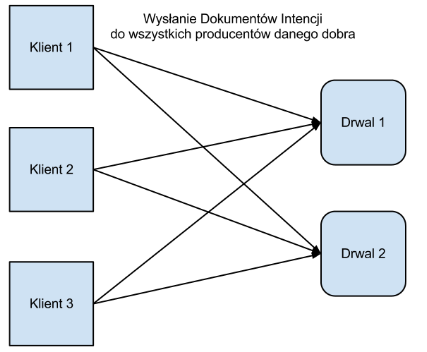
\includegraphics[scale=1]{gfx/PlatformaWymianyDobr-img2.png}
\caption{Wysłanie dokumentów intencji do wszystkich producentów danego dobra}
\label{oper1}
\end{figure}

Określają w nich typy i ilości dóbr, które dostarczają oraz jakiego typu dobra oraz cech oczekują w zamian (Rysunek \ref{oper2}).

\begin{figure}[!h]
\centering
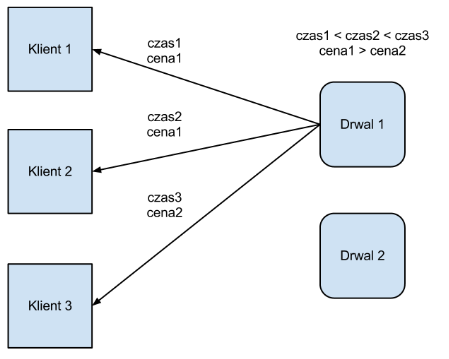
\includegraphics[scale=1]{gfx/PlatformaWymianyDobr-img3.png}
\caption{W odpowiedzi Producenci wysyłają cechy oferowanych produktów, cenę oraz czas realizacji zamówienia.}
\label{oper2}
\end{figure}

Należy pamiętać, że producenci rezerwują pewien czas na realizację zamówienia dla poszczególnych klientów, stąd też oferowany czas realizacji dla kolejnych klientów może się zwiększać.

\begin{figure}[!]
\centering
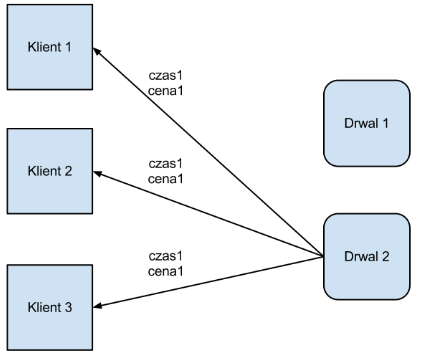
\includegraphics[scale=1]{gfx/PlatformaWymianyDobr-img4.png}
\caption{Wszyscy klienci przyjmują tą samą ofertę.}
\label{oper3}
\end{figure}

Niektórzy producenci nie rezerwują czasu dla poszczególnych klientów, co może powodować problemy w przypadku przyjęcia oferty przez wszystkich klientów (Rysunek \ref{oper3}).
\\ \\
Jeżeli producent nie będzie mógł wywiązać się z realizacji zamówienia, konieczne może być renegocjowanie kontraktu. Może to prowadzić do obniżenia reputacji producenta w przypadku niepowodzenia.

\newpage

\subsection{Implementacja}

Projekt został w całości napisany w języku JAVA w środowisku Eclipse i został podzielony na odpowiednie logiczne pakiety, które zostaną opisane w kolejnych podrozdziałach.
\\ \\
Poniżej przedstawiamy schemat architektury systemu (Rysunek \ref{schemat}) oraz pełny diagram klas przedstawiający strukturę i zależności projektu (Rysunek \ref{class_diagram}).
\\ \\
\begin{figure}[!h]
\centering
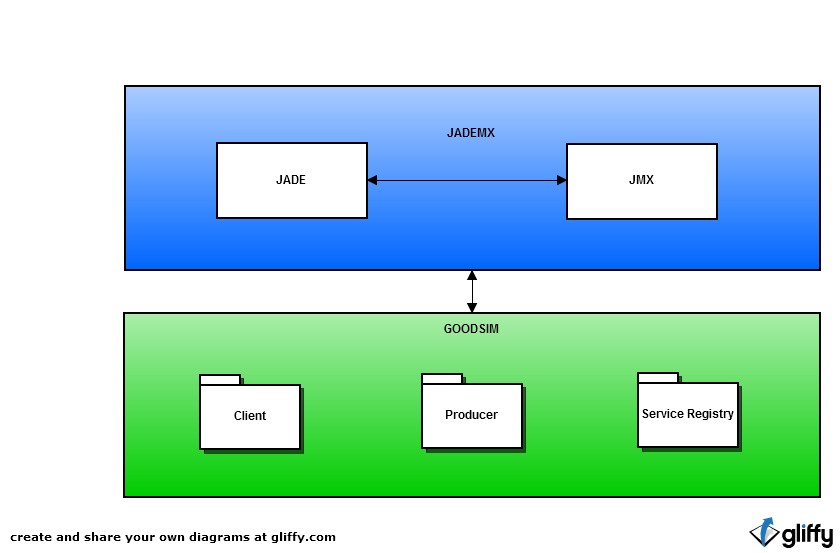
\includegraphics[scale=0.5]{gfx/goodsim.png}
\caption{Schemat architektury systemu}
\label{schemat}
\end{figure}
\\ \\
W związku z koniecznością dużego zmniejszenia diagramu na potrzeby dokumentacji, przy każdym podrozdziale znajduje się tekstowe wylistowanie zaimplementowanych klas i funkcji wraz z ich opisem.
\\ \\
Nazwy metod dobrane zostały w taki sposób, aby same się opisywały.

\begin{figure}[!]
\centering
\caption{Diagram klas}
\hspace*{-1.0in}
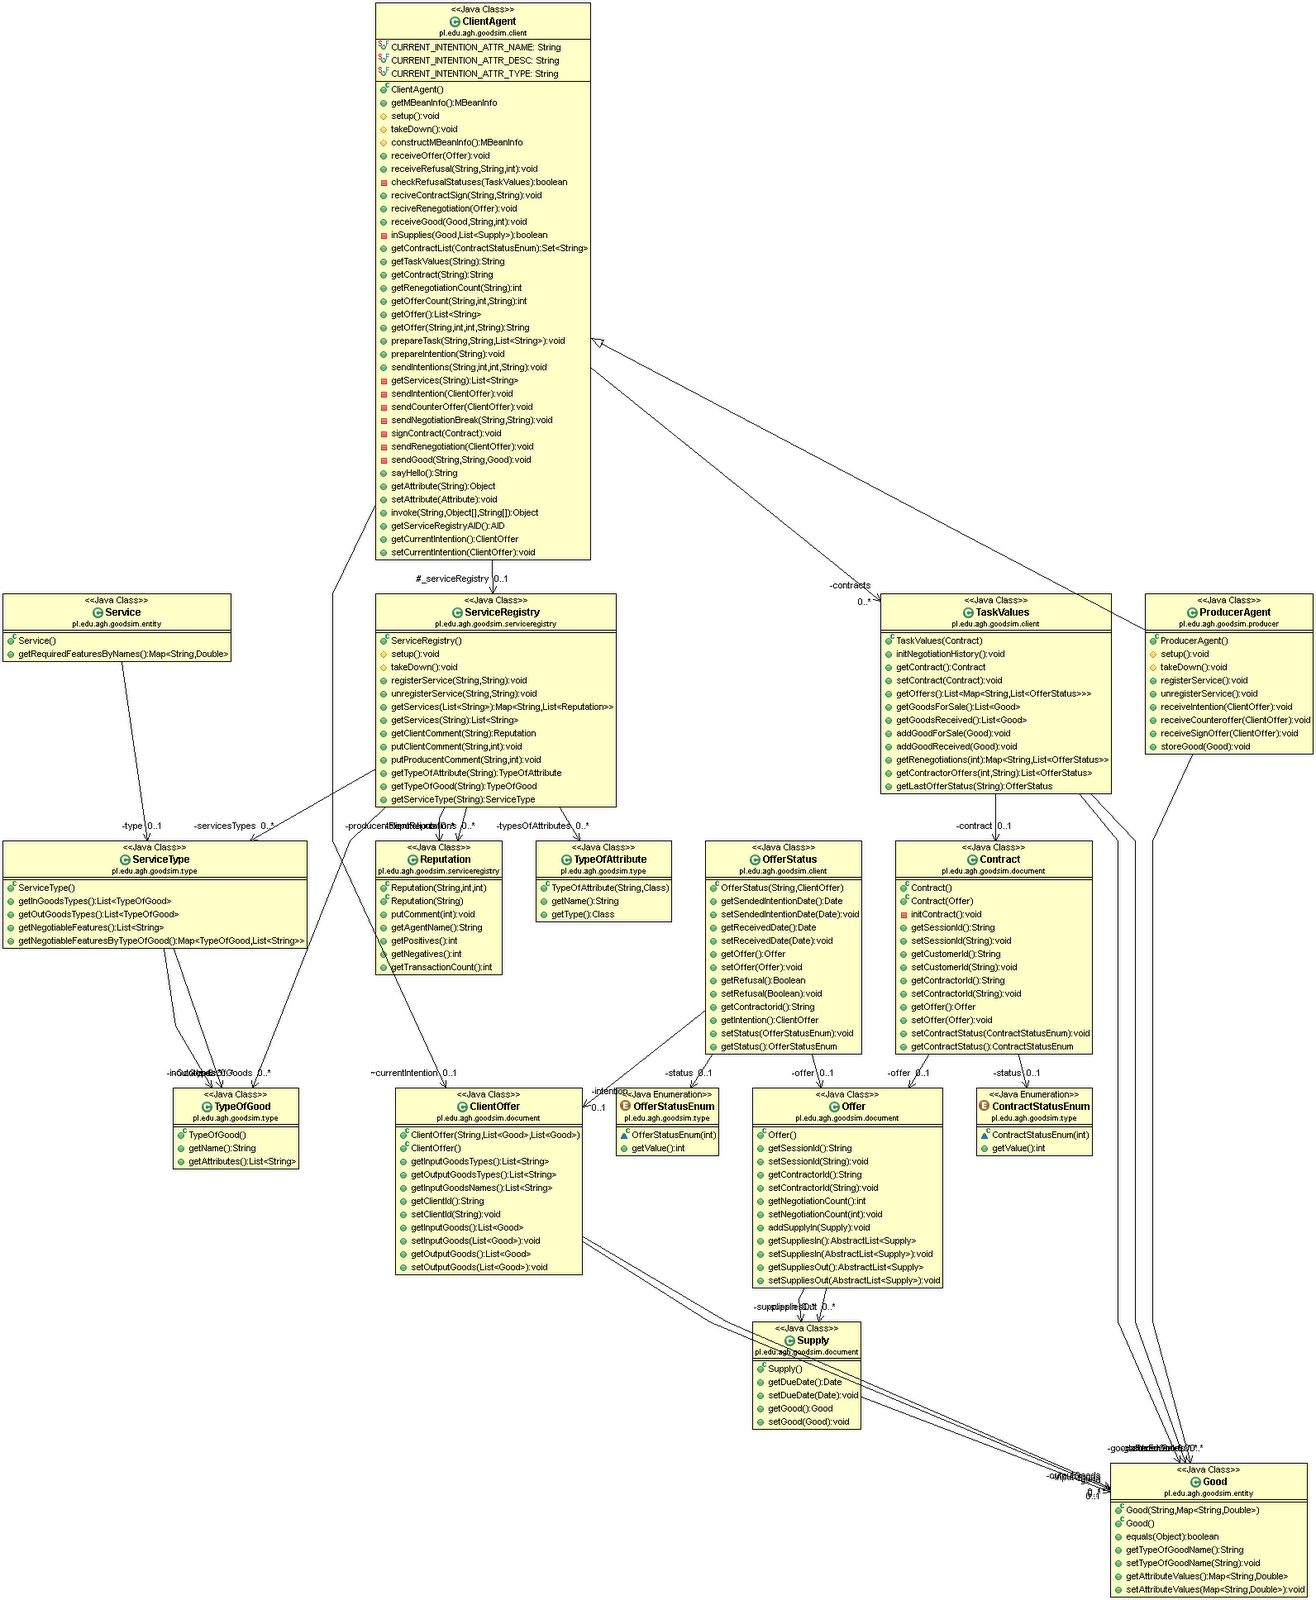
\includegraphics[scale=0.43]{gfx/PlatformaWymianyDobr-img1.png}
\label{class_diagram}
\end{figure}

\newpage

\subsubsection{Klient}

Pakiet Klienta zawiera przede wszystkim główną klasę Agenta, która implementuje odpowiedni interfejs i metody, aby mogła być użyta w środowisku JADE, a także właściwe funkcje JMX, które po uruchomieniu projektu mogą być wywoływane z konsoli JMX. Oprócz tego składa się również z klas wykorzystywanych przez Klienta do przechowywania kontraktów i historii negocjacji.
\\ \\
\textbf{ClientAgent} – agent klienta, konsument. Szerszy opis funkcji wraz z kontekstem ich wywołań znajduje się w dalszej częsci dokumentacji, na diagramie przebiegu negocjacji.
\begin{lstlisting}
MBeanInfo getMBeanInfo();
void receiveOffer(Offer offer);
void receiveRefusal(String sessionId, String contractorID, int offerCount);
void reciveContractSign(String sessionID, String contractorID);
void reciveRenegotiation(Offer offer);
void receiveGood(Good good, String sessionID, int container);
Set<String> getContractList(ContractStatusEnum status);
String getTaskValues(String sessionID);
String getContract(String sessionID);
int getRenegotiationCount(String sessionID);
int getOfferCount(String sessionID, int renegotiation, String contractorID);
List<String> getOffer();
String getOffer(String sessionID, int renegotiation, int countOffer, String contractorID);
void prepareTask(String sessionId, String mainSessionId, List<String> goodsTypes);
void prepareIntention(String intention);
void sendIntentions(String sessionId, int renegotiation, int offerNumber, String contractorId);
String sayHello();
Object getAttribute(String attribute) throws AttributeNotFoundException, 
	MBeanException, ReflectionException;
void setAttribute(Attribute attribute) throws AttributeNotFoundException, 
	InvalidAttributeValueException, MBeanException, ReflectionException;
Object invoke(String actionName, Object params[], String signature[]) throws MBeanException, 
	ReflectionException;
AID getServiceRegistryAID();
ClientOffer getCurrentIntention();
void setCurrentIntention(ClientOffer currentIntention);
\end{lstlisting}
\\ \\
\textbf{OfferStatus} – Stan oferty: 
\begin{lstlisting}
Date getSendedIntentionDate();
void setSendedIntentionDate(Date sendedIntentionDate);
Date getReceivedDate();
void setReceivedDate(Date receivedDate);
Offer getOffer();
void setOffer(Offer offer);
Boolean getRefusal();
void setRefusal(Boolean refusal);
String getContractorid();
ClientOffer getIntention();
void setStatus(OfferStatusEnum status);
OfferStatusEnum getStatus();
\end{lstlisting}
\\ \\
\textbf{TaskValues} – przechowuje cały kontekst dotyczący pojedynczego kontraktu – oferty, negocjacje, renegocjacje, producentów itd.
\begin{lstlisting}
void initNegotiationHistory();
Contract getContract();
void setContract(Contract contract);
List<Map<String, List<OfferStatus>>> getOffers();
List<Good> getGoodsForSale();
List<Good> getGoodsReceived();
void addGoodForSale(Good goodForSale);
void addGoodReceived(Good goodReceived);
Map<String, List<OfferStatus>> getRenegotiations(int renegotiation);
List<OfferStatus> getContractorOffers(int renegotiation, String contractorID);
OfferStatus getLastOfferStatus(String contractorID);
\end{lstlisting}
\\ \\

\subsubsection{Producent}

Ze względu na to, że w niektórych przypadkach Klient może stać się Producentem stworzyliśmy klasę, która dziedziczy po klasie Klienta i rozszerza go o odpowiednie dla Producenta metody.
\\ \\
\textbf{ProducerAgent} – agent producent. Posiada on wszystkie metody nalężące do agenta konsumentu, oraz poniższe:
\begin{lstlisting}
void registerService();
void unregisterService();
void receiveIntention(ClientOffer offer);
void receiveCounteroffer(ClientOffer counterOffer);
void receiveSignOffer(ClientOffer signOffer);
void storeGood(Good good);
\end{lstlisting}
\\ \\

\subsubsection{Rejestr Usług}

Rejestr usług składa się z klasy reprezentującej i implementującej agenta JADE oraz klasy, która opakowuje element reputacji w systemie.
\\ \\
\textbf{ServiceRegistry} - rejestr usług:
\begin{lstlisting}
void registerService(String serviceTypeName, String agentName);
void unregisterService(String serviceTypeName, String agentName);
Map<String, List<Reputation>> getServices(List<String> goodsTypes);
List<String> getServices(String goodTypeName);
Reputation getClientComment(String clientAgentName);
void putClientComment(String clientAgentName, int points);
void putProducentComment(String producentAgentName, int points);
TypeOfAttribute getTypeOfAttribute(String typeOfAttributeName);
TypeOfGood getTypeOfGood(String typeOfGoodName);
ServiceType getServiceType(String serviceTypeName);
\end{lstlisting}
\\ \\
\textbf{Reputation} - przechowuje reputacje klienta / producenta:
\begin{lstlisting}
void putComment(int points);
String getAgentName();
int getPositives();
int getNegatives();
int getTransactionCount();
\end{lstlisting}

\subsubsection{Encje}

Pakiet \textbf{entity} składa się z kluczowych encji obiektów, na których agenci operują w systemie.
\\ \\
\textbf{Good} – klasa reprezentująca dobro, dostępne metody:
\begin{lstlisting}
String getTypeOfGoodName(); - zwraca nazwe typu dobra
void setTypeOfGoodName(String typeOfGoodName); - ustawia nazwe typu dobra
Map<String, Double> getAttributeValues(); - zwraca wartosci atrybutow/cech dobra
void setAttributeValues(Map<String, Double> attributeValues); - ustawia wartosci atrybutow/cech dobra
\end{lstlisting}
\\ \\
\textbf{Service} - usługa:
\begin{lstlisting}
Map<String, Double> getRequiredFeaturesByNames();
\end{lstlisting}

\subsubsection{Dokumenty}

Klasy implementujące dokument intencji, ofertę oraz kontrakt.
\\ \\
\textbf{ClientOffer} – oferta klienta:
\begin{lstlisting}
List<String> getInputGoodsTypes();
List<String> getOutputGoodsTypes();
List<String> getInputGoodsNames();
String getClientId();
void setClientId(String clientId);
List<Good> getInputGoods();
void setInputGoods(List<Good> inputGoods);
List<Good> getOutputGoods();
void setOutputGoods(List<Good> outputGoods);
\end{lstlisting}
\\ \\
\textbf{Offer} – oferta:
\begin{lstlisting}
String getSessionId();
void setSessionId(String sessionId);
String getContractorId();
void setContractorId(String contractorId);
int getNegotiationCount();
void setNegotiationCount(int negotiationCount);
void addSupplyIn(Supply supplyIn);
AbstractList<Supply> getSuppliesIn();
void setSuppliesIn(AbstractList<Supply> suppliesIn);
AbstractList<Supply> getSuppliesOut();
void setSuppliesOut(AbstractList<Supply> suppliesOut);
\end{lstlisting}
\\ \\
\textbf{Contract} – kontrakt:
\begin{lstlisting}
String getSessionId();
void setSessionId(String sessionId);
String getCustomerId();
void setCustomerId(String customerId);
String getContractorId();
void setContractorId(String contractorId);
Offer getOffer();
void setOffer(Offer offer);
void setContractStatus(ContractStatusEnum status);
\end{lstlisting}
\\ \\
\textbf{Supply} - klasa opakowująca dobro wraz z datą jego wytworzenia:
\begin{lstlisting}
Date getDueDate();
void setDueDate(Date dueDate);
Good getGood();
void setGood(Good good);
\end{lstlisting}

\subsubsection{Typy}

Pakiet zawiera zaimplementowane wszystkie typy usług, dóbr, serwisów, a także statusy negocjacji.
\\ \\
\textbf{TypeOfGood} – reprezentuje typ dobra, dostępne metody:
\begin{lstlisting}
String getName(); - zwraca nazwe typu dobra
List<String> getAttributes(); - zwraca liste atrybutow typu dobra
\end{lstlisting}
\\ \\
\textbf{TypeOfAttribute} – mapuje nazwę atrybutu na jego typ:
\begin{lstlisting}
String getName();
Class getType();
\end{lstlisting}
\\ \\
\textbf{OfferStatusEnum} – status oferty:
\begin{lstlisting}
PREPARING_INTENTION(0x0), // stan poczatkowy (czekamy az przez JMX
                              // zostanie wypelniona intencja)
INTENTIN_READY(0x1),      // stan po wprowadzeniu tresci intencji
                              // przez JMX, mozna wyslac do producenta
WAITING_FOR_OFFER(0x2),   // stan po wyslaniu intencji do producenta
                              // jak przyjdzie refusal to przejscie do
                              // 0x9
OFFER_RECEIVED(0x3),      // stan po odebraniu oferty od producenta
                              // z tego stanu mozna przejsc do:
                              // 0x4, 0x6 lub 0x9
PREPAING_COUNTOFFER(0x4), // czekamy az przez JMX zostanie
                              // wypelniona kontroferta
COUNTOFFER_READY(0x5),    // stan po wprowadzeniu tresci
                              // kontroferty przez JMX, mozna wyslac i
                              // wtedy przejscie do 0x2
SIGING(0x6),              // stan po wyslaniu checi podpisania, jak
                              // zostanie odebrane refusal to przejscie
                              // do 0x9
SIGNED(0x7),              // stan po odebraniu potwierdzenia
                              // podpisania
CANCEL(0x9);
\end{lstlisting}
\\ \\
\textbf{ContractStatusEnum} - status kontraktu: 
\begin{lstlisting}
getContractStatus();
NEGOTIATION(0x1),
AWAITING(0x2),
REALISATION(0x4),
SETTLEMENT(0x8),
BEFORE_NEGOTIATION(0x10),
CLOSED(0x20),
WAIT_FOR_RESPONSE(0x40);
\end{lstlisting}
\\ \\
\textbf{ServiceType} - typ usługi:
\begin{lstlisting}
List<TypeOfGood> getInGoodsTypes();
List<TypeOfGood> getOutGoodsTypes();
List<String> getNegotiableFeatures();
Map<TypeOfGood, List<String>> getNegotiableFeaturesByTypeOfGood();
\end{lstlisting}
\\ \\

\newpage

\subsection{Komunikacja i sterowanie - JADE i JMX}

Chcąc sprawdzić działanie całego systemu i/lub modyfikować go w trakcie działania postanowiliśmy zapewnić komunikację z agentami przy pomocy technologii JMX.
\\ \\
System jest domyślnie pisany, aby działać na platformie JADE, która wspomaga budowę systemów wieloagentowych. Niestety przy jej wykorzystaniu nie ma możliwości samodzielnej rejestracji agentów w MBeanServerze, przez co technologia JMX ich ,,nie widzi''.
\\ \\
Aby połączyć oba frameworki zintegrowaliśmy nasz system do współpracy nie tylko z JADE, ale także z JADEMX, który jest środowiskiem, dzięki któremu agenci mogą udostępniać swoje atrybuty i funkcje w sposób zgodny z JMX.
\\ \\
Dzięki JADEMX możemy:
\begin{itemize}
\item skonfigurować ilość i atrybuty agentów w pliku XML,
\item uruchomić JadeMXServer, dzięki któremu możemy rejestrować Agentów,
\item uruchomić JadeFactory, które uruchamia nam agenty skonfigurowane w XML i rejestruje je w JadeMXServer
\item uruchomić ostatecznie JadeRuntime - platformę JADE, w której obecne będą nasi agenci.
\end{itemize}

Ostatecznie mamy system, którego poprawność działania możemy sprawdzać w każdym momencie, jak również możemy wpływać na zachowanie agentów, w celu testowania specyficznych przypadków.

\newpage

\subsection{Cykle życia kontraktu}

Poniżej przedstawiamy tabele, które szczegółowo przedstawiają pełny cykl życia kontraktu i jego realizacji wraz z komentarzem do każdego etapu.
\\ \\
Poruszając się od góry do dołu widzimy, który agent jest odpowiedzialny za odpowiedni stan oraz kolejność w jakiej agenci wywołują swoje funkcje.

\begin{landscape}

\begin{figure}[!h]
Rejestr usług - Rejestracja, wyrejestrowanie usługi:
\centering
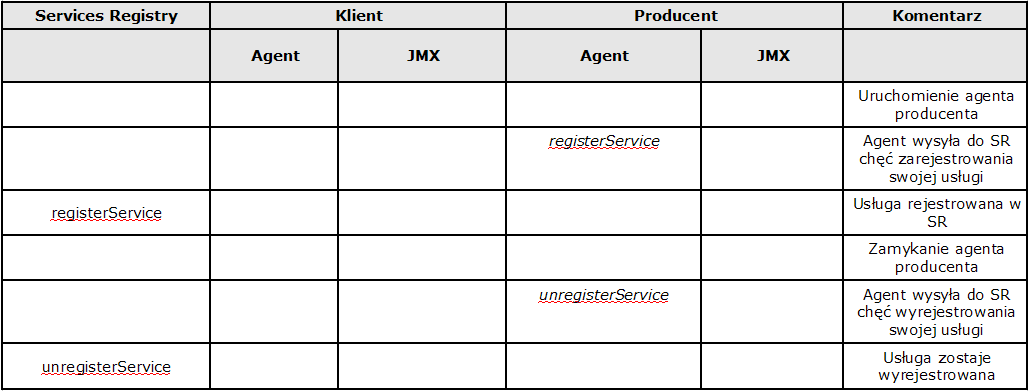
\includegraphics[width=24cm, keepaspectratio]{gfx/PlatformaWymianyDobr-img13.png}
\end{figure}

\end{landscape}

\begin{landscape}

\begin{figure}[!h]
Klient – Konsument - przebieg realizacji kontraktu przy pełnej obsłudze z konsol JMX:
\centering
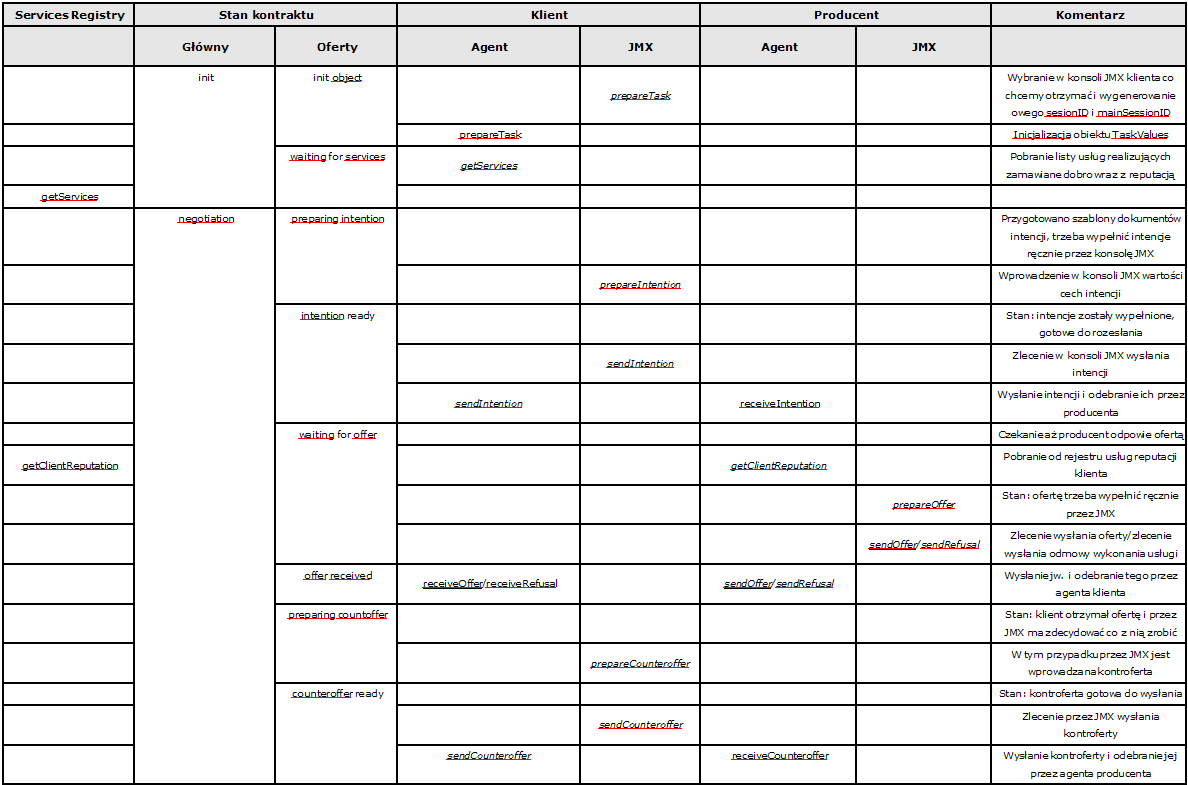
\includegraphics[width=24cm, keepaspectratio]{gfx/PlatformaWymianyDobr-img14.png}
\end{figure}

\begin{figure}[!h]
\centering
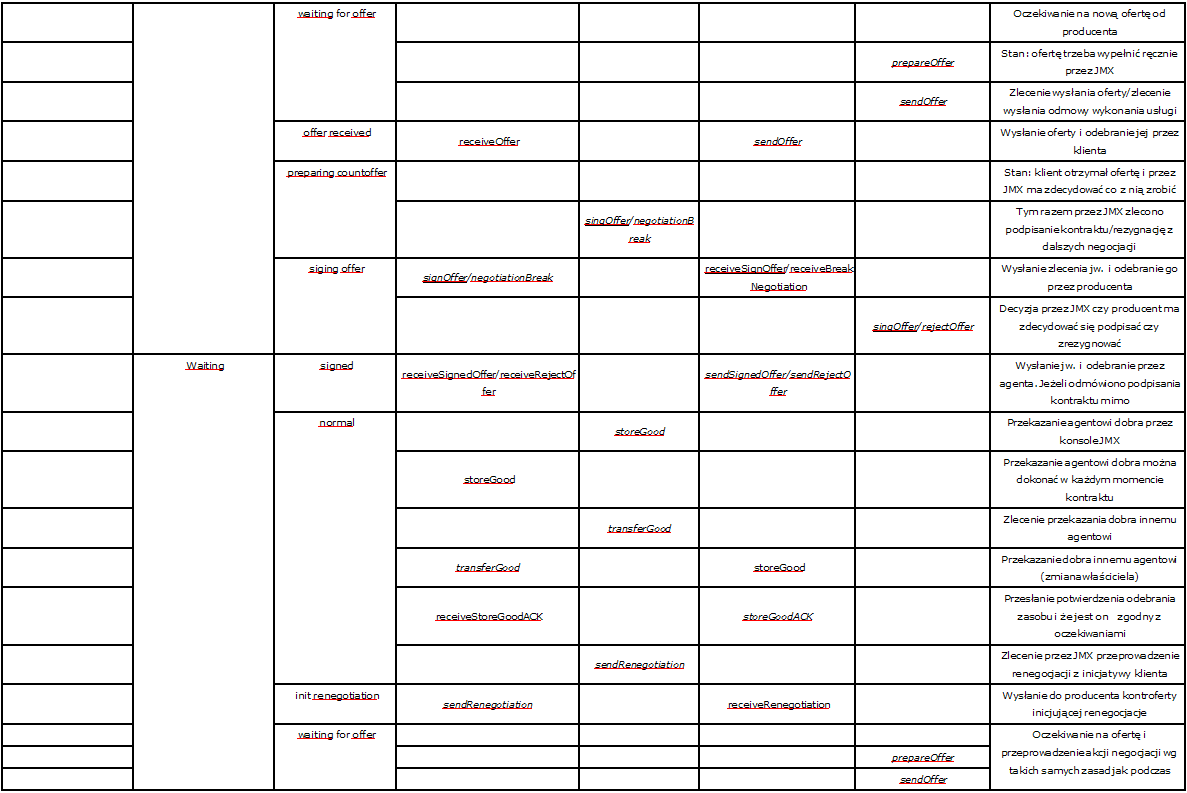
\includegraphics[width=24cm, keepaspectratio]{gfx/PlatformaWymianyDobr-img15.png}
\end{figure}

\begin{figure}[!h]
\centering
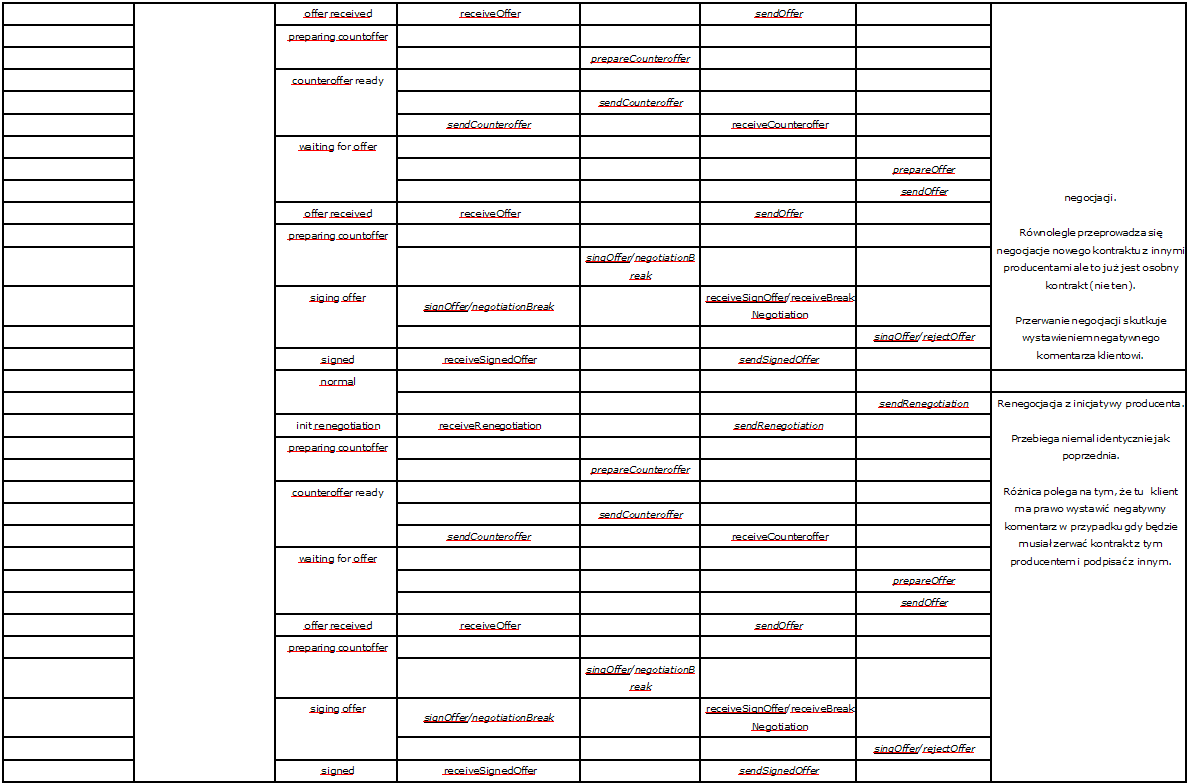
\includegraphics[width=24cm, keepaspectratio]{gfx/PlatformaWymianyDobr-img16.png}
\end{figure}

\begin{figure}[!h]
\centering
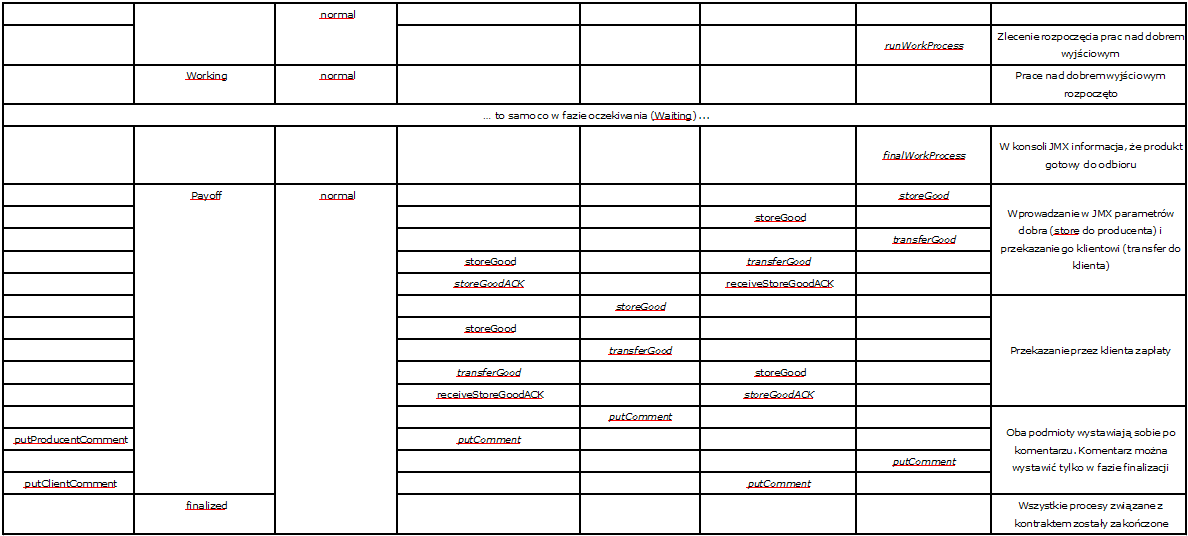
\includegraphics[width=24cm, keepaspectratio]{gfx/PlatformaWymianyDobr-img17.png}
\end{figure}

\end{landscape}

\newpage

\subsection{Instalacja i uruchomienie}

Do projektu dołączone są skrypty dla platformy Windows (install.bat, runAgent.bat) oraz Linux (install.sh, runAgent.sh).
\\ \\
\textbf{install.bat / install.sh}
\\ \\
Skrypt ten odpowiedzialny jest za zbudowanie projektu przy użyciu narzędzia Maven2, uwzględniając brak publicznego repozytorium dla archetypów jade oraz jademx. Pliki biblioteki są kopiowane do lokalnego repo, a następnie dołączane poprzez maven do projektu w celu zbudowania kompletnego archiwum .jar wraz ze wszystkimi zależnościami aplikacji.
\\ \\
\textbf{runAgent.bat / runAgent.sh}
\\ \\
Skrypt ten jest odpowiedzialny za uruchomienie podstawowej klasy platformy. Tylko poprzez takie uruchomienie, mamy możliwość uruchomienia platformy Jade wraz z rejestracją agentów w JadeMXServerze, który udostępnia metody JMX agentów.
\\ \\
W kolejnym rozdziale opisane zostały kroki uruchomienia platformy wymiany dóbr z poziomu Eclipse.

\newpage

\subsection{Demonstracja}

W celu uruchomienia przykładu z poziomu eclipse, należy użyć konfiguracji przedstawionej na rysunku \ref{conf1} i \ref{conf2}.

\begin{figure}[!b]
\centering
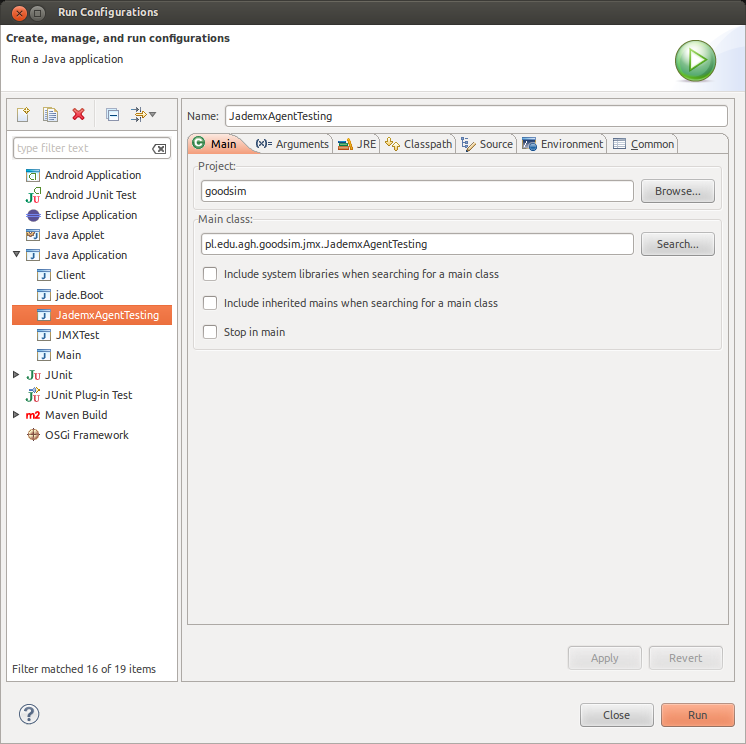
\includegraphics[scale=0.5]{gfx/PlatformaWymianyDobr-img5.png}
\caption{Konfiguracja z poziomu eclipse - główne opcje}
\label{conf1}
\end{figure}

\begin{figure}[!p]
\centering
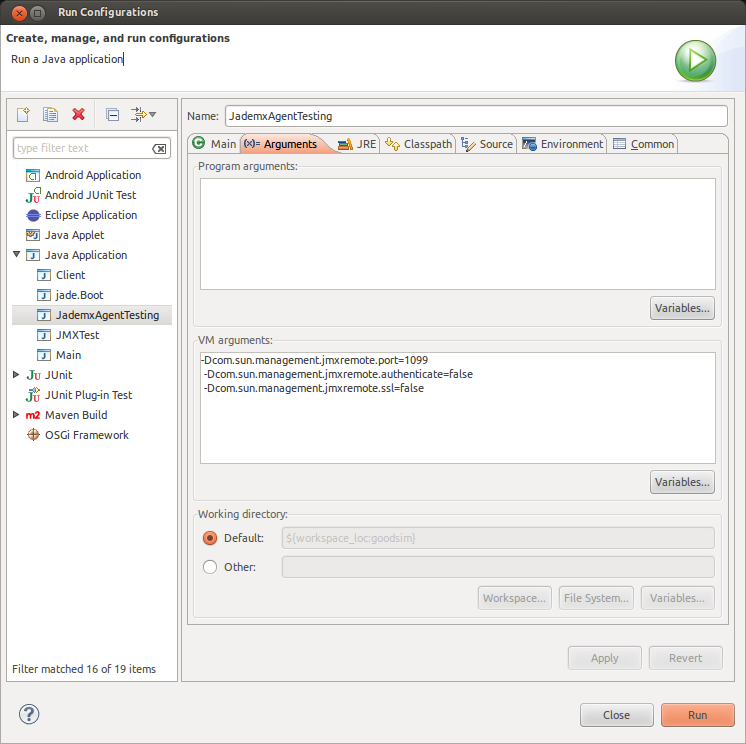
\includegraphics[scale=0.5]{gfx/PlatformaWymianyDobr-img6.png}
\caption{Konfiguracja z poziomu eclipse - parametry}
\label{conf2}
\end{figure}

\begin{figure}[!p]
Po uruchomieniu aplikacji, możemy się do niej podłączyć poprzez jconsole (Rysunek \ref{conf3}). W uruchomionym oknie, będziemy mieli dostęp zarówno do platformy agentowej jak i rezydujących na niej agentów. 
\\ \\
\begin{center}
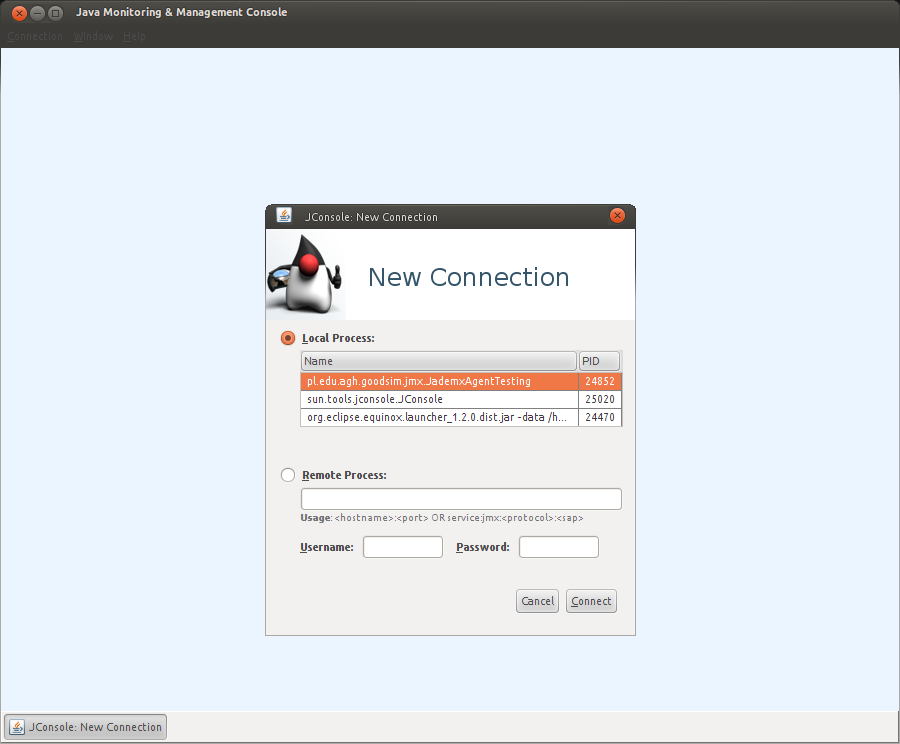
\includegraphics[scale=0.5]{gfx/PlatformaWymianyDobr-img7.png}
\caption{Konsola JMX}
\label{conf3}
\end{center}
\end{figure}

\begin{figure}[!p]
Wybierając odpowiedniego agenta, mamy możliwość wywołania na nim metody przy pomocy JMX (Rysunek \ref{conf4}).
\\ \\
\begin{center}
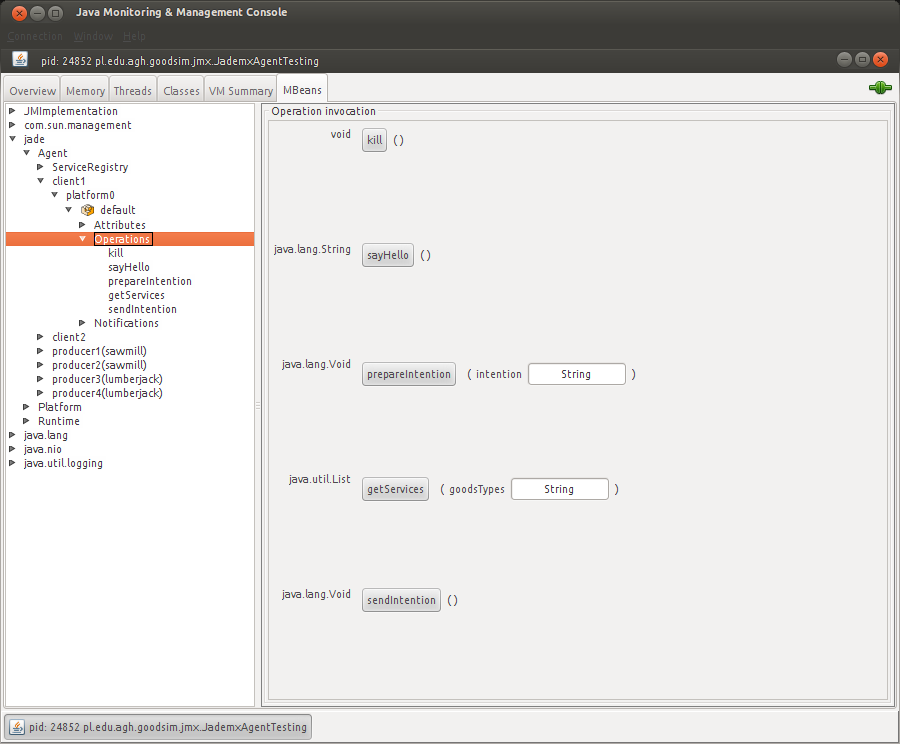
\includegraphics[scale=0.5]{gfx/PlatformaWymianyDobr-img8.png}
\caption{Przykładowe wywołanie metody JMX getServices z parametrem ,,drewno''.}
\label{conf4}
\end{center}
\end{figure}

\begin{figure}[!p]
\begin{center}
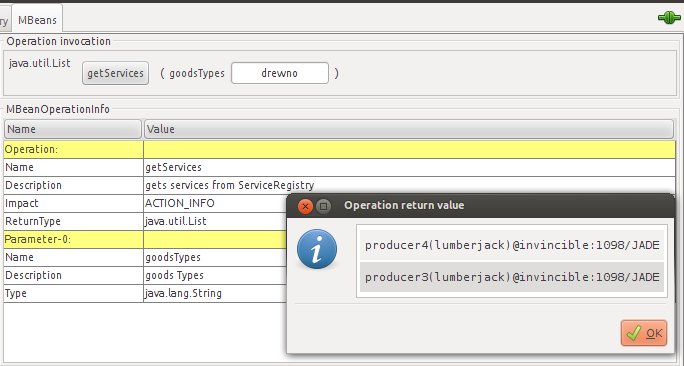
\includegraphics[scale=0.6]{gfx/PlatformaWymianyDobr-img9.png}
\caption{Widzimy odpowiedź serviceAgent w postaci listy agentów producentów oferujących typ dobra drewno.}
\label{conf5}
\end{center}
\end{figure}

\newpage

Poniżej log z przykładowego uruchomienia platformy wymiany dóbr, wraz z opisem poszczególnych kroków (Rysunek \ref{conf6}).

\begin{figure}[!p]
\begin{center}
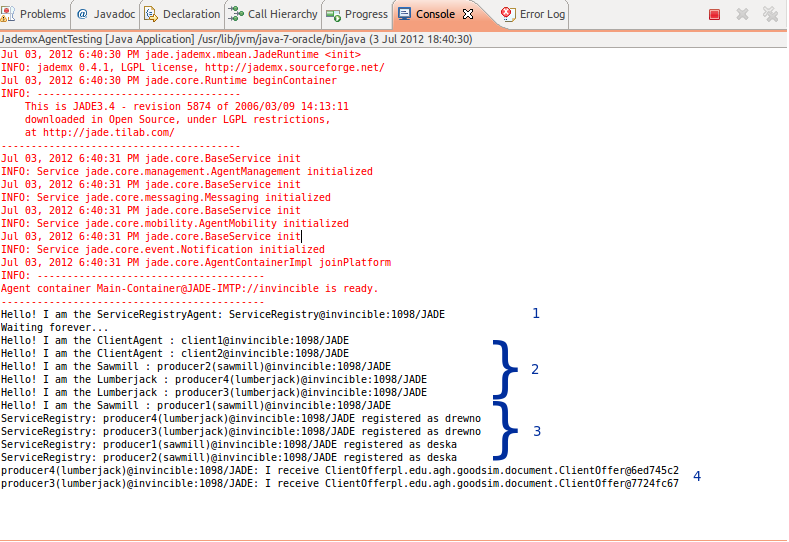
\includegraphics[scale=0.5]{gfx/PlatformaWymianyDobr-img10.png}
\caption{Wycinek logu z uruchomionej aplikacji.}
\label{conf6}
\end{center}
\end{figure}

\begin{enumerate}
\item Uruchomienie ServiceRegistry
\item Uruchomienie 2 agentów klientów oraz 4 agentów producentów (2x drwal oraz 2x tartak)
\item Rejestracja producentów w ServiceRegistry
\item Komunikat kontrolny od producentów, wywołany w odpowiedzi na odebrany od klienta dokument intencji (ClientOffer)
\end{enumerate}
\\ \\
Punkty 1-3 wywoływane są z poziomu aplikacji JADE.
\\ \\
Punkt 4 jest odpowiedzią na stworzony w kliencie, a następnie rozesłany do producentów dokument intencji. Obie te czynności wykonane są przy użyciu metod JMX, wywołanych z poziomu JConsole.

\newpage

\subsection{Podsumowanie i propozycje na kontynuację projektu}

Zrealizowany projekt dostarcza solidny fundament platformy wymiany dóbr, wraz z pełną integracją z technologiami JADE i JMX.
\\ \\
Jako kontynuację projektu, proponujemy rozbudowę istniejącego systemu o:
\begin{itemize}
\item pokrycie wszystkich funkcji agentów odpowiednimi funkcjami JADEMX
\item implementację algorytmów choreografii i orkiestracji
\end{itemize}
\\ \\
Implementacja algorytmów choreografii i orkiestracji pozwoli na w pełni dynamiczny przebieg wymiany dóbr wraz z fazami negocjacji i renegocjacji, co powinno dać ciekawe do analizy rezultaty.
\\ \\
Przykładowy przebieg wymiany dóbr po implementacji algorytmu choreografii mógłby wyglądać następująco (Rysunek \ref{choreography}):

\begin{figure}[!h]
\begin{center}
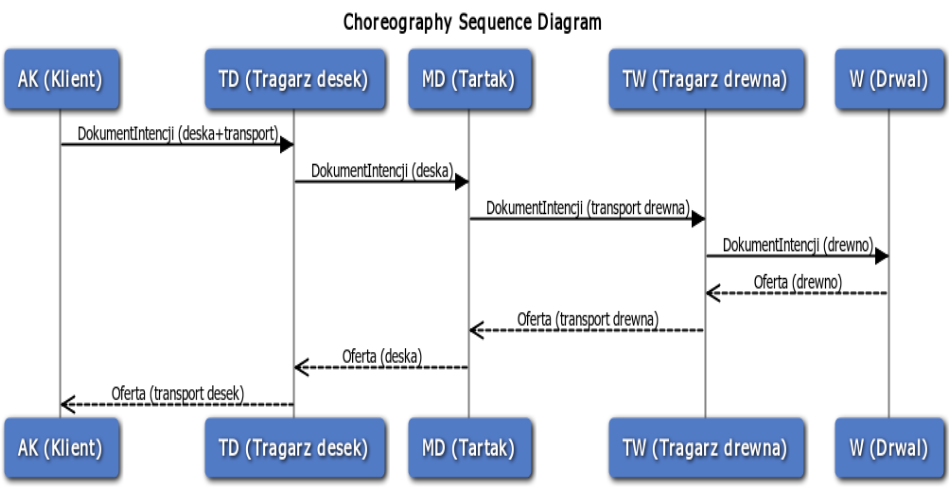
\includegraphics[scale=0.6]{gfx/PlatformaWymianyDobr-img11.png}
\caption{Diagram sekwencji algorytmu Choreografii}
\label{choreography}
\end{center}
\end{figure}

Algorytm choreografii jest z założenia kooperacyjny. Polega na widocznej globalnie interakcji, która zachodzi pomiędzy wszystkimi elementami systemu. Każda ze stron może być zaangażowana w proces wymiany wiadomości i żadna ze stron nie staje się jego właścicielem.

W przypadku algorytmu orkiestracji sytuacja wyglądałaby w następujący sposób (Rysunek \ref{orchestration}):

\begin{figure}[!h]
\begin{center}
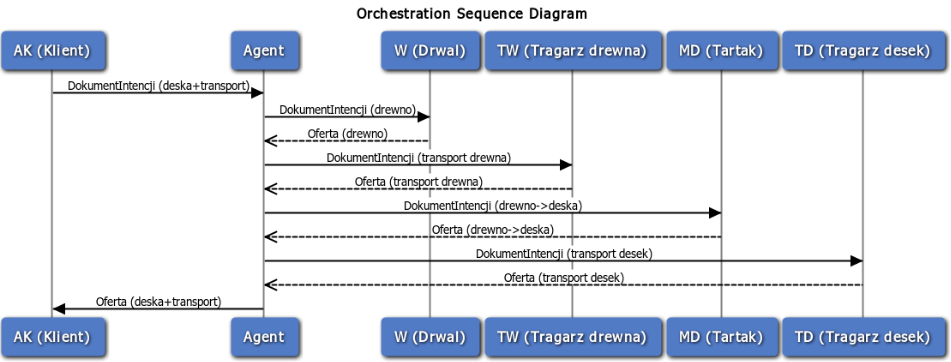
\includegraphics[scale=0.6]{gfx/PlatformaWymianyDobr-img12.png}
\caption{Diagram sekwencji algorytmu Orkiestracji}
\label{orchestration}
\end{center}
\end{figure}

Zasada działania orkiestracji jest przeciwna do algorytmu choreografii. Wyróżniamy tu jednego, centralnego Agenta, który kontroluje i pośredniczy w wymianie informacji pomiędzy elementami systemu. Orkiestracja może skutkować trwałym, wielokrokowym modelem procesu.

\newpage

\section{Bibliografia}

\begin{thebibliography}{1}
\bibitem{jade} JADE - Java Agent DEvelopment Framework -- http://jade.tilab.com/
\bibitem{jmx} JMX - Java Management Extensions Technology -- http://www.oracle.com/technetwork/java/javase/tech/javamanagement-140525.html
\bibitem{jademx} JADEMX - JMX access to JADE agents -- http://jademx.sourceforge.net/
\bibitem{maven} Apache Maven Project -- http://maven.apache.org/
\bibitem{xstream} XStream -- http://xstream.codehaus.org/
\bibitem{eclipse} Eclipse -- http://www.eclipse.org/
\end{thebibliography}

\end{document}
